\documentclass[10pt]{beamer}

\usetheme[progressbar=frametitle]{metropolis}
\usepackage{graphicx}
\usepackage{subcaption}
\usepackage{physics}
\title{Midterm update}
\date{\today}
\author{Ambrose Yim}

\begin{document}

\maketitle

\begin{frame}{Plan for today}

Recap ideas from last session

Introduce a coalition game on network model

Introduce key network concepts

Present calculations

Discuss ways to progress and model assumptions


\end{frame}


\begin{frame}[fragile]{Recap}

Each agent has a set of actions $a_i$. The actions taken by agents altogether define the `state' of the system.

We associate to each agent a utility function $u_i(a)$ evaluated on the set of it's own actions and actions of other agents.

We can define a directed network consisting of agents = nodes and a directed edge from agent $i$ to agent $j$ if the actions of agent $i$ afect the utility of agent $j$, i.e. $u_j(a_i)$. We call $i$ a `parent node' of $j$ and $j$ and child nodeof $i$; `i' is upstream of $j$, and $j$ is downstream of $i$. N.B. they may both influence each other.
\begin{figure}[b]
\centering
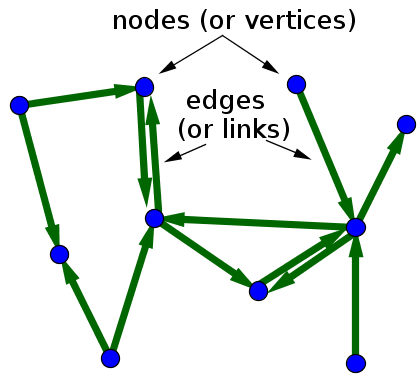
\includegraphics[height=1in]{directed_network}
\end{figure}
\end{frame}

\begin{frame}{The Socialist Agenda}

Agents form coalitions. Agents within the same coalition altruistically maximises a joint utility function defined as  $U_c(a) = \min_{i \in \mathcal{I}} u_i(a)$, so that no agent is `left behind' in the name of `progress'. Then they take action to maximise the joint utility.
$$ \max_{a \in A(C)} \min_{i \in \mathcal{I}} u_i(a) $$

Successive coalitions take action and modify the state of the system.

\end{frame}

\begin{frame}{A Simple Model: Coordination Game on Networks}
We suppose agents play a coordination game, a classic model in Game theory.

Each agent has two actions: $0$, its default state, and $1$, its compromise state.

Suppose the utility agent $i$ depends on $M$ agents.

If agent $i$ remains in its neutral state $0$, it will guaranteed to have a neutral payoff $u = 0$ independent of what the other $M$ agents do.

If agent $i$ decides to compromise, it will have a negative payoff $u <0$ if some of the $M$ agents refuses to compromise. However, if all of the other $M$ agents compromise and $i$ also decides to compromise, then $u >0$.

The `successful` end game is for all agents to mutually compromise and all obtain a positive payoff.
\end{frame}

\begin{frame}{Network model}

In our theoretical model, we only distinguish nodes by how many they affect and how many affect them, i.e. the in-degrees $j$ and out-degrees $k$. Otherwise all agents are identical.

Each node is drawn from a probability distribution of i/o-degrees $p(j,k)$. We connect them randomly by joining an outgoing stub of a node to an ingoing stub of another.

\begin{equation}
\Pr(a \to b) = \frac{k_aj_b}{m}.
\end{equation}

\begin{figure}[b]
\centering
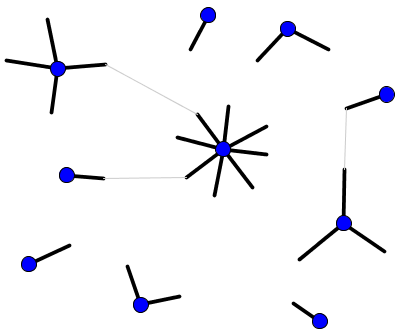
\includegraphics[height=1in]{configuration_model_algorithm.png}
\end{figure}

\end{frame}

\begin{frame}{What happens when we have coalitions?}

Suppose the system is in some initial state. We draw several nodes from the network and ask them to form a coalition.

If nodes in a coalition evaluate their joint utility function, they will realise that jointly compromising is the best strategy.

However this is only true if external nodes that the coalition depend on also decide to compromise ahead of the coalition's decision.

Otherwise the coalition would refuse to compromise, as the best outcome available is for everyone to stick to their gun and remain neutral, where $u_c = 0$.

If any one of them chooses to compromise they would make the joint utility of the coalition negative.

\end{frame}

\begin{frame}
The short story: Nodes in a coalition would only choose to compromise if the nodes that they depend on have already provided the external condition that make it favourable for them to coordinate.

This sort of dynamics is similar to network epidemic models where we have an `infection' of compromise $a=1$.

However, each unlike standard infection models, node states do not evolve synchronously; rather in this model they are only compelled to alter its state if it is included in a coalition.
\begin{figure}[b]
\centering
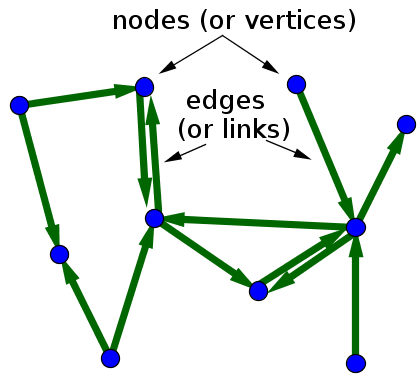
\includegraphics[height=1in]{directed_network.png}
\end{figure}
\end{frame}


\begin{frame}{Modelling decisions: Network}

We have several modelling decisions to make.

What degree distribution should we choose in our theoretical model $p(j,k)$?

What are the characteristics of the BT technology transfer `network of influence'?

What is the impact of network community/modularity structures on the dynamics?

\begin{figure}[b]
\centering
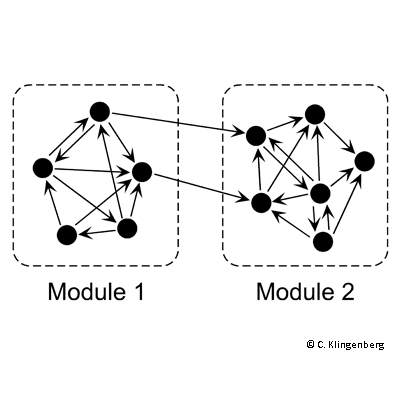
\includegraphics[height=1.5in]{community.png}
\end{figure}

\end{frame}
\begin{frame}{Modelling decisions: Seeds}
We need some `seed' nodes to compromise in the initial state. Otherwise no one would compromise. These seed nodes might represent `existing wisdom` or irrational decisions, or a misunderstanding.

How do we seed these nodes?

\end{frame}
\begin{frame}{Modelling decisions: Coalition}

How do we select coalitions?

How many nodes in a coalition? Do we select based on degree distribution?

How do we formulate a rule for deciding on an order of successive coalitions? travel along edges?

\end{frame}

\begin{frame}{What I have done}
Calculated:

Given $Q$ many seed nodes, how many nodes do they influence?

Given a random coalition of nodes, how many external nodes do they depend on?

\end{frame}

\begin{frame}{Roadmap}

Calculations on Community structure

Dynamical evolution: any critical parameters for `contagion` of compromise to sustain itself/die out?

Centrality is a seed/coalition forming condition

Simulation of dynamics on randomly generated networks, as well as empirical (social?) networks.

\end{frame}

\begin{frame}{Interlude: Percolation}

\begin{figure}[b]
\centering
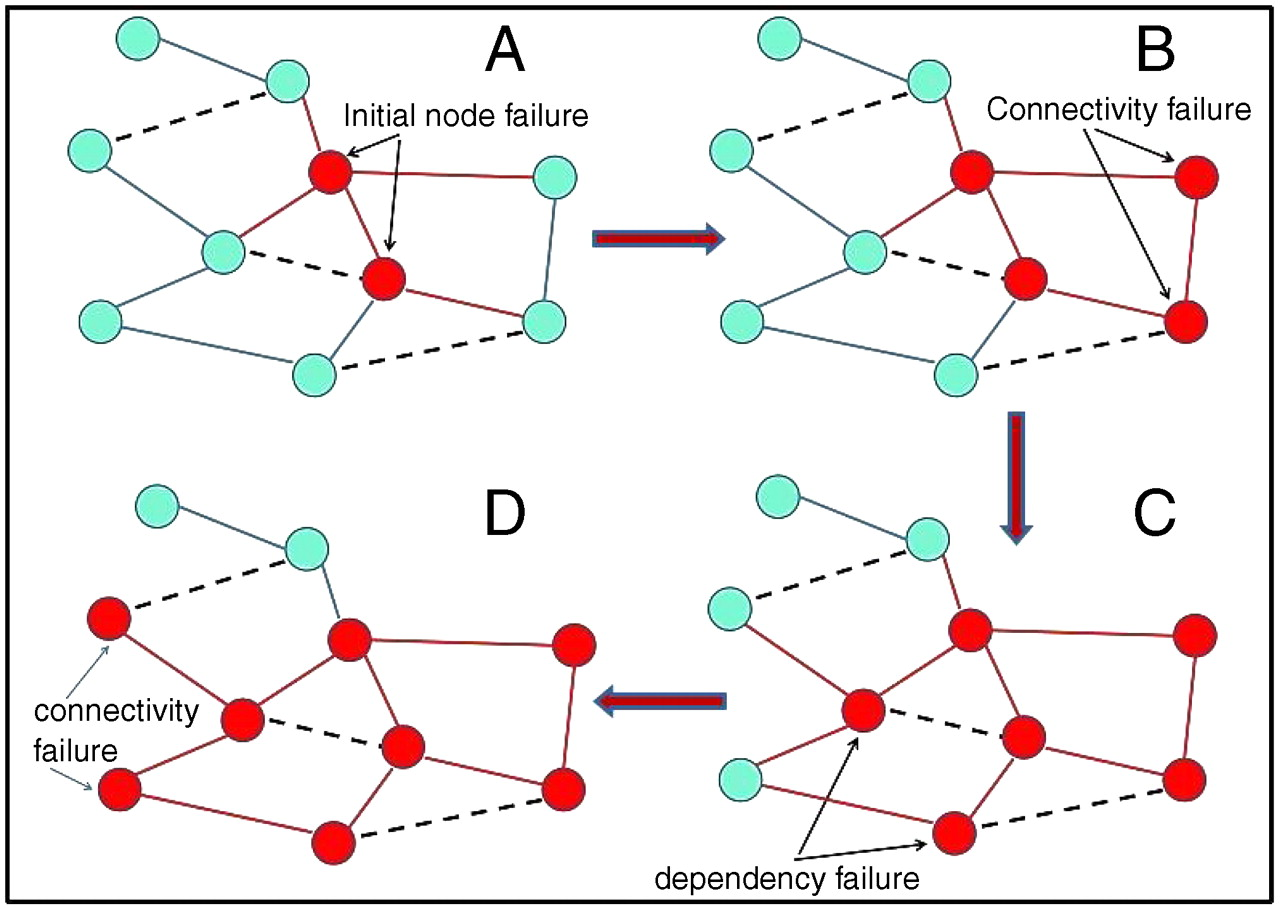
\includegraphics[width=4in]{percolation.jpg}
\end{figure}
\end{frame}


\begin{frame}{Interlude: Components}

\begin{figure}[b]
\centering
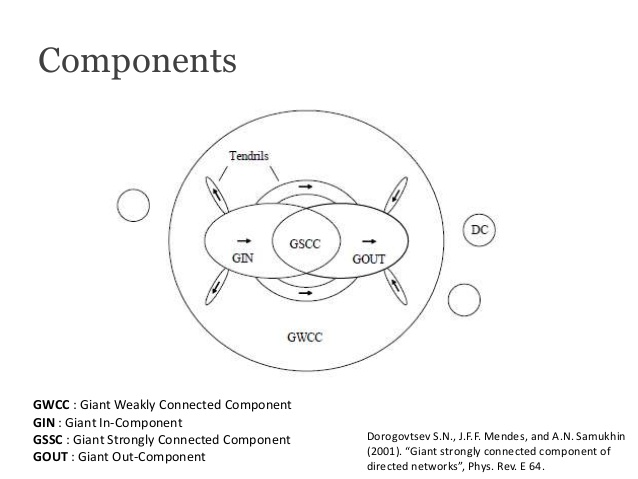
\includegraphics[width=4in]{gscc.jpg}
\end{figure}
\end{frame}
\begin{frame}{Notation}

We let $q(j,k)$ and $c(j,k)$ to be the probability that a node with i/o degrees $(j,k)$ be chosen as a seed or coalition member respectively. $r(j,k)$ is the probability that a node with i/o degrees $(j,k)$ is either a seed or coalition member. $q = \sum_{j,k} p(j,k) q(j,k)$ is the total fraction of seed nodes and $c = \sum_{j,k} p(j,k) c(j,k)$ is the total fraction of coalition nodes.

\end{frame}


\begin{frame}{No. of parents}
If I randomly sample a fraction $c$ of nodes, how many external nodes are directly upstream?

We want to calculate the average number of edges pointing to $C$ nodes if they are randomly sampled. Suppose we take away the fraction $1-c$ of nodes not in $C$. Then the degree distribution in the remaining set of nodes $C$ is
\begin{equation}
p_c'(j,k) = \sum_{J, K} p(J,K) {J \choose j} c^j(1-c)^{J-j} {K \choose k} c^k(1-c)^{K-k}.
\end{equation}
\end{frame}

\begin{frame}

The expected total in-degree of $C$ before percolation is $Nc \times \sum_{j,k} j P(j,k) = Nc\langle j \rangle$. After percolation, the expected in-degree is
\begin{align}
\sum_{j,k} j\ p_c'(j,k) &= \sum_j \sum_{J, K} p(J,K) {J \choose j} j c^j(1-c)^{J-j} {K \choose k} c^k(1-c)^{K-k} \\
&= \sum_{J} P(J) Jc \\
&= c\langle j\rangle.
\end{align}
\end{frame}

\begin{frame}

Hence after percolation the total number of edges remaining is $Nc^2\expval{j}$. Therefore the number of in-edges from the nodes outside the coalition is $\eta = Nc\langle j \rangle - Nc^2\langle j \rangle = Nc(1-c) \langle j \rangle$. The maximum is $\eta (1/2) = N\expval{j}/4$: the in-edges from nodes outside the coalition constitute a quarter of all edges; another quarter goes in the other direction, out of the coalition, and the remaining half are edges within the two groups.

\end{frame}

\begin{frame}

Suppose now $c = c(j,k)$. For a non-trivial sampling, the degree distribution of the coalition embedded in the pre-percolation network is
\begin{equation}
p_c(j,k) = \frac{c(j,k)p(j,k)}{c}.
\end{equation}
Thus prior to percolation, the average in-degree in the coalition is
\begin{equation}
\frac{\sum_{j,k} j p(j,k) c(j,k)}{\sum_{j,k} p(j,k) c(j,k)} = \frac{\expval{jc}}{c}.
\end{equation}
So the total number of in-edges in the coalition prior to percolation is
\begin{equation}
Nc \frac{\expval{jc}}{c} = N\expval{jc}.
\end{equation}
\end{frame}

\begin{frame}
Now we percolate the network such that only nodes in the coalition remain, where each node with i/o-degree $(j,k)$ has a survival probability of $c(j,k)$. Consider in-an edge pointing to a surviving node. The edge could only survive if the parent of the edge is also a coalition node. The probability that the parent node is a node with out-degree $k'$ is $k'p(j',k')/\expval{k}$, and the probability that such a node is also in the coalition is $k'p(j',k')/\expval{k} c(j',k')$. Thus the probability that the in or out edge survives percolation is
\begin{align}
\Pr(\text{in-edge survives}) &= \sum_{j',k'} \frac{k'p(j',k')}{\expval{k}} c(j',k') = \frac{\expval{ck}}{\expval{k}} \\
\Pr(\text{out-edge survives}) &= \sum_{j',k'} \frac{j'p(j',k')}{\expval{j}} c(j',k') = \frac{\expval{cj}}{\expval{j}}
\end{align}
\end{frame}

\begin{frame}
Thus in calculating the average in-degree of the coalition after percolation we replace $c$ in the case of uniform percolation with $\expval{ck}/\expval{k}$ or $\expval{cj}/\expval{j}$ in appropriate places, and also update the i/o-degree distribution of the coalition embedded in the original network $p(j,k)$ to $p_c(j,k)$, we now get
\begin{equation}
\sum_{j,k} j p_c'(j,k) = \frac{\expval{jc}\expval{kc}}{c\expval{k}}.
\end{equation}
Thus the total number of in-edges in the coalition surviving percolation is
\begin{equation}
Nc \frac{\expval{jc}\expval{kc}}{c\expval{k}} = N\frac{\expval{jc}\expval{kc}}{\expval{k}}.
\end{equation}
So the total number of in-edges pointing to the coalition from outside the coaltion is
\begin{equation}
 N\expval{jc} - N\frac{\expval{jc}\expval{kc}}{\expval{k}} = N\expval{jc}\qty(1-\frac{\expval{kc}}{\expval{k}}).
\end{equation}
\end{frame}

\begin{frame}{No. of strictly downstream children}
We define the \emph{ideal} coalition, or strictly downstream set of seed $Q$ to be the set of nodes satisfying
\begin{equation}
\iota \in C \qq{iff} Q \cup C \to \iota,
\end{equation}
If we choose nodes strictly downstream of the seeds to form a coalition, those nodes will agree to compromise.
\end{frame}
\begin{frame}
Since each in-edge independently chooses its parent, the probability that the node has parent nodes of i/o-degrees $\qty((j_1, k_1), \ldots, (j_{j-1}, k_{j-1}))$ (labelled by some arbitrary indexing of edges) is
\begin{equation}
\Pr(\qty(j_e, k_e)_{e=1}^{j} \ \lvert \ j,k) = \prod_{e=1}^j\frac{k_e}{\expval{k}} p(j_e, k_e).
\end{equation}
Thus the probability that such nodes have either seed or coalition parents is
\begin{equation}
\Pr(\qty(j_e, k_e)_{e=1}^{j},\ Q\cup C \to \iota \ \lvert \ j,k) = \prod_{e=1}^j\frac{k_e}{\expval{k}} p(j_e, k_e)r(j_e, k_e).
\end{equation}
\end{frame}


\begin{frame}
Summing over all degree configurations, and observing that sum of products = product of sums
\begin{align}
\Pr(Q\cup C \to \iota \ \lvert \ j,k) &= \prod_{e=1}^j\qty(\sum_{k_e,j_e})\prod_{e=1}^j\frac{k_e}{\expval{k}} p(j_e, k_e)r(j_e, k_e) \\
&= \qty(\sum_{k',j'}\frac{k'}{\expval{k}} p(j', k')r(j', k'))^j = \qty(\frac{\expval{rk}}{\expval{k}})^j
\end{align}

We observe that $\frac{\expval{kr}}{\expval{k}}$ is nothing more than a constant (given some choice of $q$ and $c$).
\end{frame}

\begin{frame}
If we define the \emph{ideal} coalition such that
\begin{equation}
\iota \in C \qq{iff} Q \cup C \to \iota,
\end{equation}
then
\begin{align}
c(j,k) &= \Pr(\iota \in C \ \lvert \ d(\iota) = (j,k), Q)\\
 &=  \Pr(Q \cup C \to \iota \ \lvert \ d(\iota) = (j,k), Q) \\
 &= \qty(\sum_{k',j'}\frac{k'}{\expval{k}} p(j', k')r(j', k'))^j = \qty(\frac{\expval{kr}}{\expval{k}})^j.
\end{align}
and thus $c(j,k) = c(j)$ is independent of $k$, i.e. probability of a node with i/o-degrees $(j,k)$ is in the coalition is independent of the node's out degree. If we let $c(j=1) = \gamma$, where $1 \geq \gamma > 0$,
\begin{equation}
c(j) = \gamma^j \quad \forall j = 1,2, \ldots.
\end{equation}
\end{frame}

\begin{frame}
N.B. $c(0) = 0$. Furthermore if we assume that $Q$ was a random sample of the graph, where a node with i/o degrees $(j,k)$ is sampled with probability $q(j,k)$, then
\begin{equation}
r(j,k) = c(j) + q(j,k) - c(j)q(j,k).
\end{equation}
Then we can solve for $c(j)$ from a self-consistency solution:
\begin{align}
\gamma &= \sum_{k,j}\frac{k}{\expval{k}} p(j, k)\qty(q(j,k) + c(j)\qty(1-q(j,k)))\\
&= \frac{\expval{qk}}{\expval{k}} + \sum_{j=0}c(j)\sum_{k=1}\frac{k}{\expval{k}} p(j, k)\qty(1-q(j,k)) \\
&= \frac{\expval{qk}}{\expval{k}} + \sum_{j=1}\gamma^j\sum_{k=1}\frac{k}{\expval{k}} p(j, k)\qty(1-q(j,k))
\end{align}

\end{frame}
\begin{frame}
If we have $q(j,k) = q$ and let $s(j) = \sum_{k=1}\frac{k}{\expval{k}} p(j, k)$,
\begin{align}
\gamma &= q + \qty(1-q) \sum_{j=1}\gamma^{j}s(j)\ ; \qand \\
q &= \gamma \qty(\frac{1-\sum_{j=1} \gamma^{j-1}s(j)}{1-\sum_{j=1} \gamma^js(j)})
\end{align}
We notice that there is are obvious trivial solutions $(\gamma, q) = 0$ and $\gamma(q=1) = 1$, while $q$ is undefined for $\gamma = 1$ and $s(0) = 0$ (where $p(j=0, k \neq 0)=0$). $q$ becomes undefined if
\begin{equation}
q > 1 - \frac{\expval{k}}{\expval{jk}} = q_c.
\end{equation}
\end{frame}

\begin{frame}
In other words, if we have more than $Nq_c$ seed nodes $Q$, the size of the set of nodes $C$ that is downstream of $Q$ or $C$ is the whole network. This is automatically satisfied if $\expval{kj} = \expval{k}$, loosely meaning that nodes on average have one in-edge and one out-edge i.e. the network is very close to a chain. In addition, this critical value coincides with with the threshold percolation value for the destruction of the \textbf{giant connected component} after removing a fraction $q$ of nodes from the network.
\end{frame}

\begin{frame}
Suppose $p(j,k) = p(j)p(k) \qand p(j) \sim j^{-\beta}$

\begin{figure}[b]
\centering
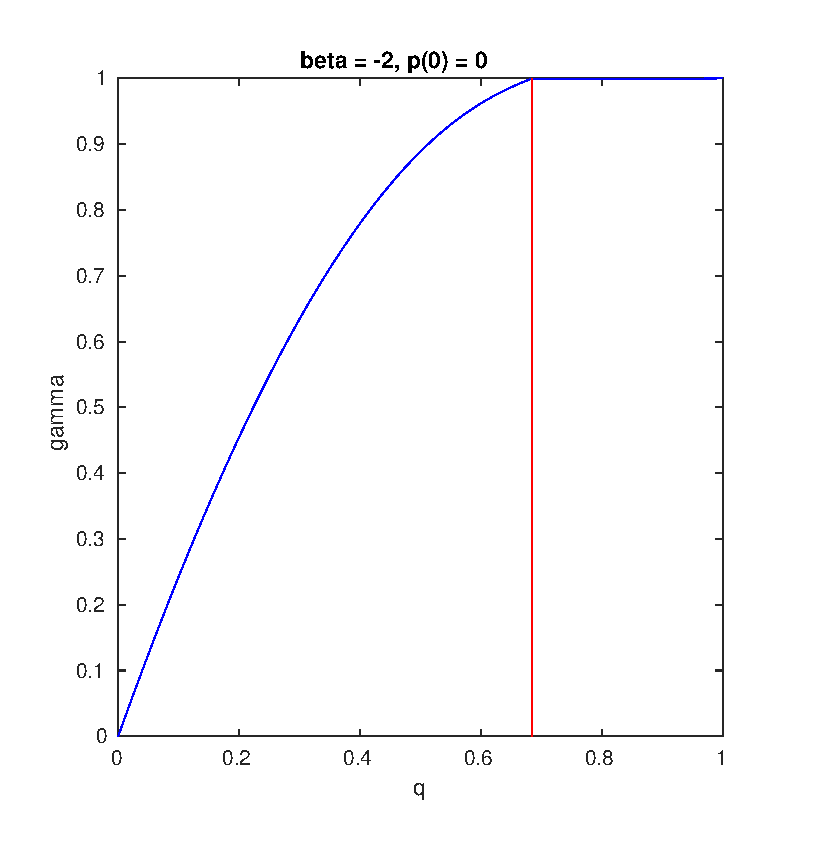
\includegraphics[height=2.6in]{beta2.eps}
\end{figure}
\end{frame}


\begin{frame}
Recall $q_c = 1 - \frac{\expval{k}}{\expval{jk}} = \frac{\expval{j} - 1}{\expval{j}}$

\begin{figure}[b]
\centering
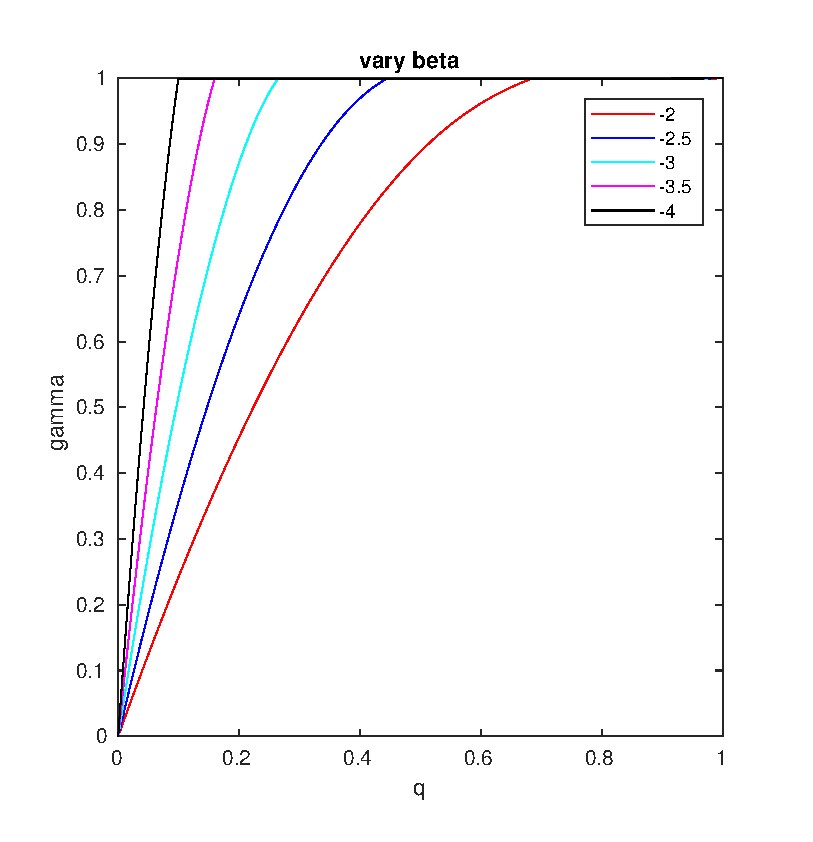
\includegraphics[height=2.6in]{beta_vary.eps}
\end{figure}
\end{frame}

\begin{frame}
Suppose now $p(j =0) \neq 0$
\begin{figure}[b]
\centering
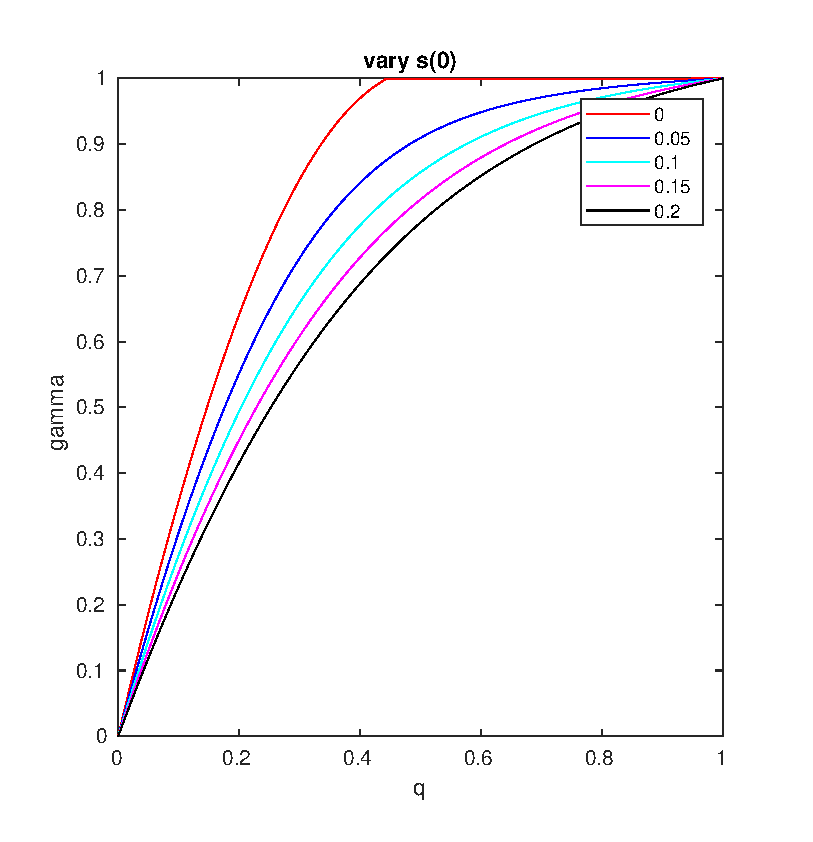
\includegraphics[height=2.6in]{s0_vary.eps}
\end{figure}
\end{frame}

\begin{frame}{Community Structure}
A probabilistic network model for networks that are `modular` is the stochastic block model.

The set of nodes are evenly partitioned into $B$ `blocks' labelled by $\beta$

For two nodes $a$ and $b$ in blocks $\beta$ and $\beta '$ respectively, the probability of $a \to b$ is
\begin{equation}
\Pr(a \to b \ \lvert \ a \in \beta,\ b \in \beta ') = \frac{k_a j_b}{m}\omega(\beta, \beta ').
\end{equation}
where $\omega(\beta, \beta')$ is a weight that controls the probability of a node in $\beta$ begin the parent of a node in $\beta'$.



\end{frame}

\begin{frame}{Results Highlights}

Coordination Game played by coalition on network = contagion

Fraction upstream nodes of a coalition $= \frac{\expval{jc}}{\expval{j}}\qty(1 - \frac{\expval{kc}}{k})$.

Fraction of nodes of degrees $(j,k)$ strictly downstream of seed is $c(j) = \gamma^j$.

As we grow coalition the value of $\gamma = \frac{\expval{rk}}{\expval{k}}$ evolves. Is it possible to reach $\gamma = 1$ in time $\order{N}$?

Entire network becomes strictly downtream when initial seed exceeds $q_c = 1 - \frac{\expval{k}}{\expval{jk}}$.

\end{frame}

\begin{frame}{Points for discussion}
Validity of modelling assumptions: large (infinite) network, identical nodes, coordination game.

How meetings are organised at BT. Coalition dynamics.

\end{frame}

\end{document}
